\chapter{Introduction}

Violent events throughout history have had a substantial role in directing the geological and biological evolution of our planet. At least five times in the past 540 million years half or more of all species have been wiped out in a short space of time. Distinctions in the variety and quantity of fossil species alongside cratering records reveals times of ancient catastrophes \citep{1986gss..conf..338S}. Signs of global environmental downturn and large scale disruption of photosynthesis are evident in tree ring data \citep{doi:10.1146/annurev.ea.16.050188.000445} and an observed global `gap' in Early Triassic coal deposits \citep{doi:10.1130/0016-7606(1996)108<0195:GCGBPT>2.3.CO;2}.

Until quite recently, geologists were conditioned against seeing any evidence of sudden and abrupt major crises. Originating from the paradigm of uniformitarianism introduced by \cite{lyell1830principles}, there was the view that all geological phenomena can be explained by processes we see today, extrapolated over much longer timescales. This picture held for 160 years, with all mass extinctions of living species in Earth's history thought to be engendered by causes of a terrestrial nature.  Because of this, a more gradualistic cause for the signatures of mass extinctions manifested in the geological record was at first favoured - with the consensus being that Earth's timeline has been characterised by low magnitude, high frequency events. 

However more recently the role of catastrophic events of high magnitude and low frequency has been brought to the fore, by the recognition that one the most well-known mass extinctions of 66 million years ago coincided with an impact event. Recent studies by \cite{Renne684, Schulte1214} into the Alvarez hypothesis \citep{Alvarez1095} have upheld the conclusion that an impactor brought about the Cretaceous-Tertiary (KT) mass extinction that caused the downfall of the dinosaurs and 70\% of all species at the time.

The reality of major extraterrestrial impacts of comets and asteroids has been demonstrated in modern times. The Tunguska impact of 1908 was an enormous airburst that took place over sparsely populated Eastern Siberia. The explosion was responsible for flattening 2,150 square kilometres of forest and liberated 10-15 Mt TNT equivalent of energy \citep{1975PEPI...11....1B}. Work by \cite{Kolesnikov2010} suggests that the Tunguska bolide was of a cometary origin.

The fragmentation and subsequent collisions with Jupiter of comet Shoemaker-Levy 9 in July 1994 was the first direct observation of a collision between Solar System objects. The series of fragments impacting Jupiter generated fireballs thousands of kilometres in size, easily visible to small telescopes on Earth \citep{2004jpsm.book..159H}. 

In February 2013, a large airburst of a small asteroid 18 m in diameter \citep{2013Natur.503..238B} occurred over the Chelyabinsk region in Russia, with the shockwave causing substantial building damage and injuring over 1500 people. This event was widely observed by infrasound, seismic and video recording instruments, providing a detailed insight and led to an increased global awareness into the potential damage that even relatively small impacts from comets and asteroids can cause.   
%SOMETHING TIE THIS IN TO NEOs IN GENERAL

\section{Taxonomy of Comets and Asteroids}
\label{sec:taxonomy}

Most of the Earth-impacting meteoroid flux is made up of near-Earth asteroids and short-period comets (SPCs). Near-Earth asteroids and SPCs are collectively known as near-Earth objects (NEOs). SPCs have an orbital period $P < 200$ yrs - comets with longer orbital periods are known as long-period comets (LPCs). NEOs are defined somewhat arbitrarily as having a perihelion $q < 1.3$ AU from the Earth.

The orbital period distribution of all known comets continues smoothly over the 200 year threshold - a choice of threshold that somewhat reflects the low quantity of accurately resolved comet orbits in the past. Therefore whilst not necessarily subsumed under the category of NEOs, LPCs also present an Earth impact  threat. Due to their long orbital periods, close approaches and potential impacts with Earth cannot be calculated reliably in advance. Also, these objects can only be easily detected if their perihelion passage coincides with the present epoch. Both facts lead to the omission of LPCs in modern NEO observation programmes - a salient point discussed in more detail in \S~\ref{sec:comet_impact_hazard}.

Long viewed as distinct objects with regard to composition and orbital characteristics - the definition separating asteroids and comets has been blurred in recent years. The traditional, fundamental differences between asteroids and comets can be attributed to the differences in their composition.

Asteroids are rocky/metallic bodies dominated by refractory materials and contain few volatile compounds (e.g. water ice). Asteroids appear stellar and point-like in the sky (with angular diameter $< 1"$), mostly physically located in the asteroid belt, with aphelia typically within 2.2 and 3.2 AU from the Sun. Most asteroids located in the asteroid belt have relatively circular orbits, with low eccentricities ($e < 0.4$) and are found within a narrow range from the ecliptic, with inclinations of less than 30$^\circ$ \citep{2002AJ....123.2070T}. 

Comets, on the other hand, are usually thought to be mostly icy planetesimals built around cores of dust mixed with ice, formed beyond the snow line in the nascent Solar System. Comets are found on elongated elliptical orbits, some with orbital periods extending to thousands of years. In the Solar System, comets are not expected to follow the plane of the ecliptic, unlike other Solar System bodies. While SPCs may have relatively small orbits and low eccentricities by comparison, LPCs vary in the extreme - isotropically distributed in orbital inclination and are located much further away from the Sun \citep{DEMEO2008436}. The populations of short and LPCs correspond to the Oort cloud and Kuiper Belt -  now recognised as two primary primordial sources for comets in the Solar System \citep{2017ApJ...845...27N} (see \S~\ref{sec:origin_of_comets}). 

Comets exhibit gravitationally unbound and diffuse atmospheres (comae) that entrain grains of dust and ice, and tails due to gas production from a solid nucleus \citep{1950ApJ...111..375W}. However, there exists practical constraints in determining whether or not an object possesses a coma due to limitations in seeing and instrument sensitivity. Weak outgassing can lead to faint comae, further blurring the observational distinction between these objects. Therefore, while an object may have the requisite physicochemical properties of the cometary type, there is no necessary guarantee that it may exhibit cometary behaviour. As a result, orbital parameters can help further distinguish small bodies even further.
%http://iopscience.iop.org/article/10.1086/383208/pdf for difficulty distinguishing

%\clearpage

The Tisserand invariant with respect to Jupiter, $T_J$, is a popular discriminant to help separate asteroids and comets, solely on their dynamical properties \citep{1995EM&P...68...71C}. \clearpage The parameter is defined as,

\vspace{-2ex}
\begin{equation}
    T_J = \dfrac{a_J}{a} + 2\left( {(1-e^2)\dfrac{a}{a_J}} \right)^{1/2} \cos(i)~,
\label{eq:tiss_param}
\end{equation}

where $a$, $e$, and $i$ are the semi-major axis, eccentricity and inclination of the orbit of a small body respectively, while $a_J$ = 5.2 AU is the semi-major axis of the orbit of Jupiter. Derived from Jacobi's integral, the Jovian Tisserand parameter characterises the strength of the gravitational interaction between strong planetary perturber Jupiter and a small body. Eqn.~\eqref{eq:tiss_param} is derived assuming the orbit of Jupiter is both circular and non-inclined. Because the orbit of Jupiter is eccentric and slightly inclined, $T_J$ is not strictly conserved, and is described as a quasi-constant of orbital motion away from close encounters with Jupiter or the Sun. The evolution of $T_J$ is much slower than the evolution of $P$ and therefore is a more favoured parameter for the dynamical classification of Solar System objects. 

\begin{figure}[t!]
    \centering
    \vspace{-3ex}
    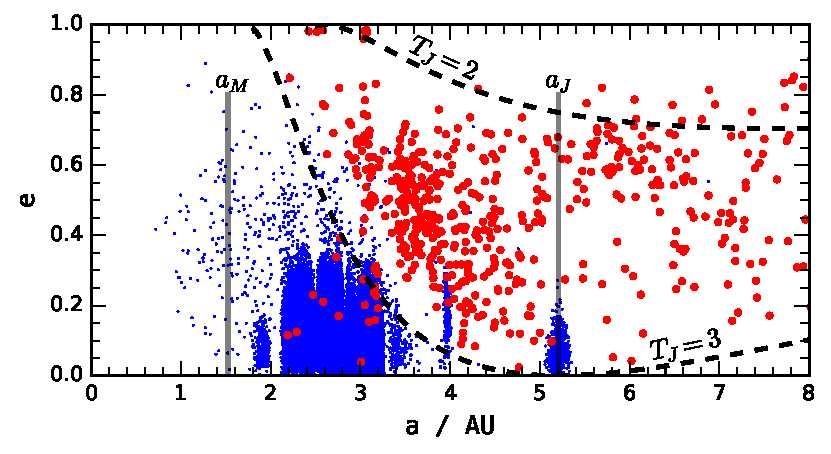
\includegraphics{a_e_tisserand.pdf}
    \caption[Tisserand parameter plot for known asteroids and comets]{A plot of the semi-major axes against eccentricities of the first 50000 numbered asteroids (blue) and all comets (red) catalogued by the IAU MPC. Lines of constant $T_J$ (with inclination $i=0$) are plotted as dashed lines, and the semi-major axes of Mars $a_M$ and Jupiter $a_J$ are marked with vertical grey lines.}
    \label{fig:tiss_param}
\end{figure}

Asteroids from the main belt typically have $T_J > 3$, meaning that (excluding resonance), they orbit independently from the strong direct effects of Jupiter. Jupiter itself has  $T_J = 3$. Objects with  $T_J < 3$ are strongly tied with Jupiter and can therefore have low velocity interactions with it. Adopting the nomenclature from \cite{1987PAICz..67...21C}, Jupiter Family Comets (JFCs) generally have $2 < T_J < 3$ and $P < 20$ yrs, and Halley Family Comets (HFCs) have $T_J < 2$ and $P < 200$ yrs. The JFC population is tightly concentrated in orbital space with short orbital periods and low inclinations, while the HFC population is more dispersed in their orbital periods and inclination - alluding to different origins.

\cite{1996ASPC..107..173L} expanded comet taxonomy further by defining nearly-isotropic comets (NICs) as having $T_J < 2$, and comets with  $T_J > 2$ as ecliptic comets (ECs). Long term integrations of comets orbits have shown that the majority of comets with $P < 200$ yrs remain in one of these two classes in their dynamical lifetimes. These classes are therefore regarded as dynamically significant, reflecting perhaps the existence of the origin of these two comet populations (see \S~\ref{sec:origin_of_comets}).

Fig.~\ref{fig:tiss_param} shows that most asteroids have $T_J>3$, and most comets have $T_J<3$. However, there are many asteroids scattered from the main belt with $T_J < 3$ and several comets with  $T_J > 3$ (including comet 2P/Encke), meaning that these boundaries are far from impermeable. The majority of asteroids in the $2 < T_J < 3$ range belong to either the Jupiter Trojan asteroid ($a \sim 5.2$ AU) or the Hilda asteroid ($a \sim (3.7-4.2)$ AU) populations.

While the terms `asteroid' and `comet' are still commonly used to describe small bodies in the Solar System, major advances since the 1990s have led to the acceptance that these are not clearly separate classes of objects, and instead part of a continuum \citep{1989aste.conf..880W, 2002aste.book..669W}. Far from being a tidy dichotomy - it has been increasingly hard to classify particular objects as rates of discovery increase.

%Several comets have been misidentified and provisionally designated as asteroids, only later to be reclassified as comets, for example the initial observation of object P/Smirnova-Chernykh as asteroid 1967 ED \citep{Rickman1985}. The recent discovery of `Oumuamua, the first interstellar object observed to pass through our Solar System - prompted much discussion as to whether the object was of a cometary or asteroidal origin. It is currently argued by \cite{2017arXiv171109599R} that on dynamical grounds, `Oumuamua is a dormant cometary nucleus, but many conflicting discussions continue \citep{2017arXiv171107535F, meech2017brief}. %The resulting nomenclature problem has currently been resolved by a new designation scheme for interstellar objects \citep{2017arXiv171206721G}.

The overlap and increased uncertainty in the taxonomy of Solar System small bodies in recent times is due to our rapidly changing understanding of comets and asteroids. Recent advances in our understanding owe much to the increasingly sensitive detections that we can now achieve compared to just a few years ago.

%Centaurs, Damacloids 

\vspace{-.5ex}
\section{Cometary Reservoirs}
\label{sec:origin_of_comets}

%https://arxiv.org/pdf/1712.03961.pdf explanation of how comet got frozen into oort cloud orbits

The median dynamical lifetime of SPCs is $4.8\times10^4$ yrs \citep{1991AJ....102..787L}, and $6\times10^5$ yrs for LPCs \citep{1979IAUS...81..277W}. This suggests that for a steady state comet population to be guaranteed, all observed comets are recent arrivals into the inner Solar System. They must be continually resupplied from permanent reservoirs far beyond the planetary region.

The existence of cometary reservoirs and the implications of the infall of comets into the inner Solar System has been investigated since the 1950s \citep{1950BAN....11...91O, 1951PNAS...37....1K}. The distant Oort cloud was first identified as a primary storage of $\sim10^{12}$ NICs larger than 1 km in diameter, with an inner edge of the cloud being $(1-2)\times10^4$ AU. Objects in this system are barely gravitationally bound to the Solar System and therefore are sensitive to galactic disturbances \citep{1981AJ.....86.1730H}. The large semi-major axes of NICs alongside the isotropic distribution of orbital inclinations supports the need for a spherically structured Oort cloud.

Numerical integrations of orbits from the location of the Oort cloud by \cite{1988ApJ...328L..69D} found that the source for ECs had to be located elsewhere in the Solar System, and that a cometary source consisting of low inclination objects would be a more appropriate candidate in producing the orbits of many observed ECs.

Following the discovery of several comet-sized objects by the HST \citep{1995ApJ...455..342C}, it has since been concluded that ECs are sourced from a trans-Neptunian reservoir - made up of a cometary belt known as the Kuiper Belt, as well as an associated circumstellar disc known as the `scattered disc' \citep{1997Sci...276.1670D}. These reservoirs are thought to be natural remnants of the outer regions of the solar nebula, hosting $\sim10^{10}$ comets with modest inclinations and eccentricities that are located just beyond the orbit of Neptune with aphelia in the range 35-50 AU \citep{1993AJ....105.1987H}. Theoretical and observational studies of the Kuiper Belt and Scattered Disc have identified this region as the source for most JFCs, while most HFCs originate in the Oort cloud.

Research by \cite{2005Natur.435..466G} has shown that rapid migration of the giant planets in the early beginnings of the Solar System may have dramatically changed the location of comet populations, such that present reservoirs do not necessarily reflect their true origin and formation location.

Differentiating between the dynamical classes of comets and subsequently identifying reservoirs of cometary bodies in the Solar System are both important steps in order to conduct realistic simulations of the orbital migration of these bodies in the Solar System. Doing this allows one to gain a greater understanding of the evolution of comets from their reservoirs and into the inner Solar System.

\vspace{-.5ex}
\section{The Comet Impact Hazard}
\label{sec:comet_impact_hazard}

%Involving telescopes such as LSST and Pan-STARRS

As of April 2018, initiatives by NASA have detected a total of 18101 NEOs\footnote{https://cneos.jpl.nasa.gov/stats/totals.html}, with SPCs making up less than 1\% of this total. The latest generation of telescopic surveys including Pan-STARSS \citep{1538-3873-125-926-357}, CSS \citep{1998BAAS...30.1037L} and NEOWISE \citep{2011ApJ...743..156M} are currently dominating NEO discoveries. The majority of the largest potentially hazardous and globally-devastating objects are now known - with over 90\% of objects meeting the NEO criteria and having a diameter larger than 1 km. For the comets in the current catalogued NEO population, their variable levels of activity means that their sizes remain mostly unknown.

It is important to address the current shortfalls of leading NEO studies. A white paper published by NASA that detailed various ground and space-based survey programmes for the detection of NEOs \citep{united2007near} failed to address numerous important classes of hazardous objects from outer space - including LPCs and objects with a short warning time. While such a preoccupation into observable objects with short-period orbits is understandable with regards to statistical risk and the limitations of current technology, it could lead to a hubristic belief in current planetary defence efforts, yielding a biased or incomplete risk inventory. Even after an exhaustive search for NEOs in the vicinity of Earth with the latest technologies, there remains the residual impact risk from a class of objects that may represent the dominant impact threat to humanity.

%what we're doing now in term of pho prevention - predominately asteroids because that's all we can find with current tech

Comparatively little attention thus far has been given to the threat of LPCs. While it is perhaps correct that objects presently covered the NEO definition represent the vast majority of the perceived impact problem - there remains the fact that as little as two years notice may accompany the arrival of a LPC impactor with Earth (due to high relative velocities), if any warning at all \citep{1994hdtc.conf..221M}. 

A striking example of this is in 1983, when comet C/1983 H1 was discovered merely two weeks before its close encounter of 0.0312 AU with the Earth. %WHY NOT DETECTED?
%SOMETHING HERE ABOUT ONLY DETECTED AT JUPITER AND WHY?
%need to explain why LPC are still dangerous, but we just don't know anything about them until they reach Jupiter
Studies by \cite{1997NYASA.822...67W} have stated that the most probable impact velocity for LPCs with Earth to be of $\sim (56-58)$ km$\,$s$^{-1}$, energetic enough for an exceptionally devastating impact.
%however really unlikely! then lead onto comet showers

Understandably, the prevailing NEO surveys focus on cataloguing dangerous cis-Jovian objects that are liable to cross Earth's orbit. However, the resulting NEO population statistics may be responsible for an inadequate reflection of the true impact hazard.

A study by \cite{2004MNRAS.355..191N} discussed the absence of thousands of HFCs along with their associated decay products - orders of magnitude fewer than what has been predicted by considerations of the dynamical evolution of LPCs captured from the Oort cloud. To account for the discrepancy they proposed the existence of inert, extremely low albedo HFCs in Earth-crossing orbits. Such a large population of extremely dark comets would be undetectable by current NEO programmes.

The cratering patterns found on Earth and the Moon suggest the volume of near-Earth objects (NEOs) is episodic in nature \citep{1998ncdb.conf...21N, 1979Natur.282..455N}. Evidence for temporally correlated comet showers has given rise to the hypothesis of `coherent catastrophism' (otherwise known as the Shiva Hypothesis \citep{Rampino1996}).

Previous studies have suggested that, on timescales relevant to modern times, the existence of periodic impacts may pose the prime impact hazard \citep{ASHER19941}. Suggested mechanisms for this coherent catastrophism include the arrival of giant cometary bodies, known as Centaurs, from dynamically unstable regions moving towards the inner Solar System \citep{2015A&G....56f6.24N}. The disintegration of such a Centaur could introduce many objects with short-period, potentially Earth-crossing orbits. The fragmentation of an especially massive Centaur could mean that the total mass of these objects would be $10^{2}-10^{3}$ times the mass of the near-Earth asteroid system. As well as the threat of prolonged periods of bombardment from the rapid introduction of Centaur comet fragments, there are questions about the consequences of Earth's passage through a debris trail, and the large injection of mass into the zodiacal cloud from a cometary breakup - resulting in the dust influx to Earth acquiring climatically devastating increases in optical depth \citep{2001MNRAS.321..463N, 2015MNRAS.448...27N}.

Additional sudden replenishment of the NEO-population could also involve the injection of comets into short-period regimes, as a result of perturbations of the Oort cloud by gravitational interactions with the mid-plane of the galaxy, large molecular clouds, or passing stars.

The postulated mechanisms for a dramatic introduction of cometary bodies into NEO orbits allows us, at a minimum, to recognise the greater complexity of the cometary hazard in contrast to the asteroidal hazard, as well as its more extensive effects.

%Current impact mitigation strategies are currently based upon the assumption that at the very minimum, decades of warning can be made available following the discovery of a potentially hazardous object.  

%Full mapping of the LPC and dark comet population is beyond current technology.
%one argument is that comet make up such a small part of population anyway
%disingenuous to suggest that - because coherent catastrophism. quiescent stage of comets then come all at one


%summary is: comet threat is not being taken seriously. one way to maybe better out understanding on how to mitigate this is to run sims and work out the risk this way, and where abouts they come from

%finally - if the comet threat is real... what can be feasibly achieved with current technology

%“Shiva Hypothesis”
%http://adsabs.harvard.edu/abs/1996EM%26P...72..441R
%http://adsabs.harvard.edu/abs/1998HiA....11..246R
%http://adsabs.harvard.edu/abs/1985JGRS...90...24G

%breakup of Centaurs/comet splitting
%work by \cite{1972IAUS...45..283P} found that interactions between comets and the asteroid belt, or interactions at perihelion or at the ecliptic are not or are weakly correlated with comet splitting events. Splitting appears randomly distributed along a comet's orbit.

%The Centaurs are dynamically intermediate between the Kuiper Belt andthe Jupiter Family Comets. We here define Centaurs as objects with periheliaq > aJ and semimajor axes a < aN , where aJ = 5.2 AU and aN = 30 AUare the semimajor axes of Jupiter and Neptune, respectively (Jewitt and Kalas1998). By this definition, there are currently (October 2002) 42 known Centaurs,including the prototype 2060 Chiron, also known as 95P/Chiron (a = 13.6 AU, e= 0.38, i = 15 deg). Most appear asteroidal but five have been observed to showcomae and thus are also properly recognized as comets  http://citeseerx.ist.psu.edu/viewdoc/download?doi=10.1.1.485.4044&rep=rep1&type=pdf


%Unlike most other natural disasters, cosmic impacts can be both predicted and prevented. If sufficient warning is available, we can develop technologies to de#ect the object or evacuate the imp


%The asteroid/comet impact hazard is a realistic threat to the human population. The magnitude of the risk is at least as great as that of many other natural hazards, with the potential of an individual occurrence being orders of magnitude greater than any disaster ever experienced

%http://adsabs.harvard.edu/abs/1980A&A....85..191W physical loss of LPCse
\vspace{-.5ex}
\section{Research Goals}
\vspace{-.5ex}

In order to lend appropriate credence to the comet threat - numerical integrations can help quantify the hazard. The complexity of the various postulated facets of the comet impact hazard detailed in \S~\ref{sec:comet_impact_hazard} are in general related to the fact that these particular threats cannot be readily detected by modern instrumentation. This is either due to current technological limitations, or because comet-impact activity with Earth may possibly be at a stage of temporary quiescence - a lull before a huge introduction of comets into the near-Earth environment. Numerical integrations allow one to simulate Solar System dynamics, and apply the results to observations if possible.%dont like this paragraph at all please reword

There have been considerable advances in N-body numerical simulations in recent years, driven by the growing availability of low-cost computing resources and increasingly advanced numerical codes. Because of this, computer models that incorporate our current understanding of comet dynamics will make important strides in enabling us to envisage a range of possible future scenarios for planet Earth - and evaluate how best to mitigate a possible threat without having to make any prior real-world observations.

%STRUCTURE OF REPORT
%research goals
%dynamical transfer mechanisms
%Opik, 1963

In this paper, we perform N-body simulations of cometary bodies in the Solar System. In \S~\ref{chap:method}, we describe our numerical method. We report on the simulation results and discuss their implications in \S~\ref{chap:results}. \S~\ref{chap:mitigation} discusses how best to mitigate cometary remnant impacts and explores a predictive model approach to identifying hazardous cometary material from current observations. We conclude with a summary of our results in \S~\ref{chap:conclusion}, ending with a discussion on the implications these have on the present state of planetary defence policy.
